\subsubsection{DSP Klassen}

DSP klassen har til formål at indsamle og behandle den data, som alle sensorerne leverer. Klassen er designet så den er meget skalerbar, da den kan opsættes til at gemme de alt imellem én og flere hundrede seneste målinger for hver sensor. Ligeledes kan den justeres til hvor mange af de gemte målinger der skal være valide, for at måleresultatet er gyldigt og kan sendes til DevKit8000 frem for en fejlmeddelelse. Ud over denne vurdering er klassen designet, så den foretager et gennemsnit af alle de gemte datapunkter for en bestemt sensor, og gemmer den i en variabel (fx \texttt{temp}) der er klar til at blive hentet ud af klassen og sendt direkte til DevKit8000.

\begin{figure}[ht]
\centering 
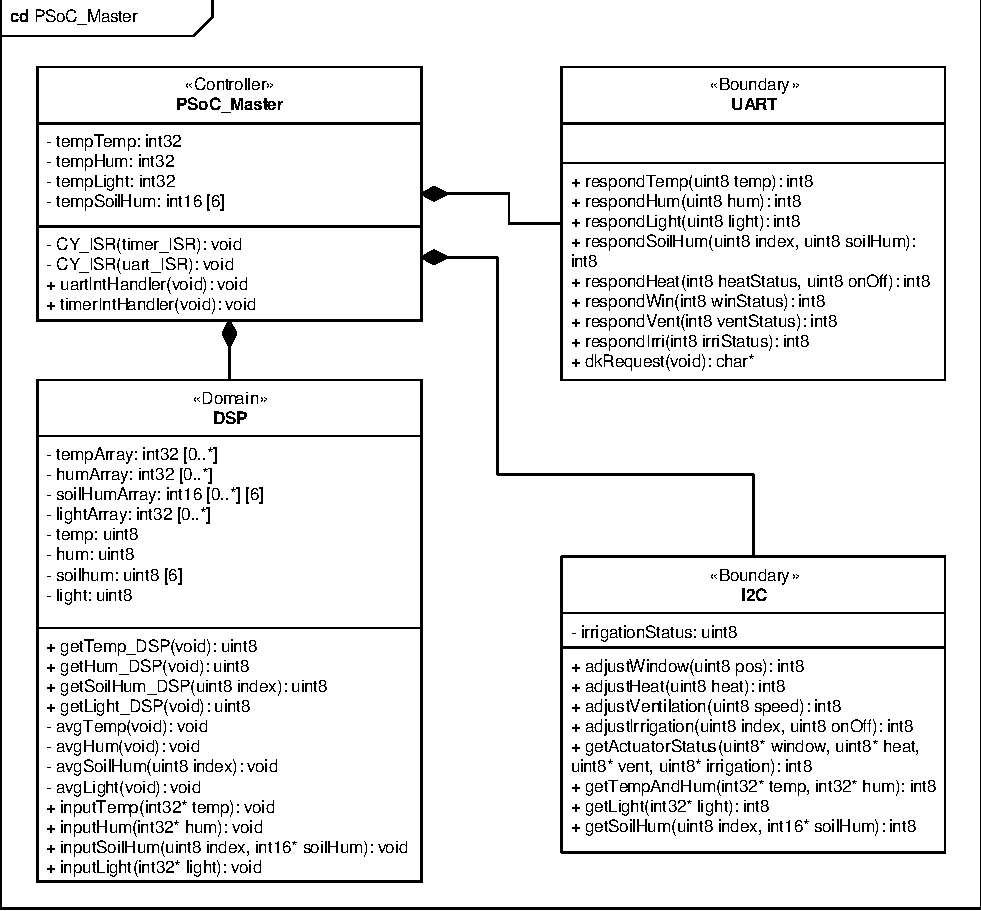
\includegraphics[width=\textwidth * 2/5, trim=15 13 268 182, clip=true] {../fig/cd_PSoC_master.pdf}
\caption{DSP klassen.}
\label{fig:DSP_klasse}
\end{figure}

På Figur \ref{fig:DSP_klasse} ses et klassediagram over DSP klassen. Der er private datamembers både i form af arrays og almindelige variable til at gemme hhv. rå sensordata og klargjorte data. Det kan ses, at \texttt{soilHumArray} er et to-dimensionalt array, da det herved er nemmere at implementere behandlingen af jordfugt-data ved for-løkker.

Vejen for et datapunkt ind og ud af klassen kan beskrives ved et par punkter. Her er et eksempel med temperaturen:

\begin{enumerate}\itemsep1pt \parskip0pt \parsep0pt
\item Den målte temperaturdata hentes direkte fra sensoren og gemmes i DSP klassen ved at kalde \texttt{inputTemp()} metoden fra PSoC Master klassen (styret af en timer).

\item Når \texttt{inputTemp()} kaldes, gemmes datapunktet i \texttt{tempArray} og den private metode \texttt{avgTemp()} kaldes herefter automatisk.

\item Metoden \texttt{avgTemp()} kontrollerer, om der er nok valide datapunkter, tager gennemsnittet over alle punkterne i \texttt{tempArray}, konverterer data'en til formatet der passer til UART protokollen og gemmer resultatet i \texttt{temp}.

\item Når DevKit8000 anmoder om temperaturen, kan \texttt{getTemp\_DSP()} blot kaldes for at få den færdigbehandlede temperatur.

\end{enumerate}

Det detaljerede design med klassebeskrivelser m.m. kan findes i afsnit \ref{P-sec:DSP_class_design} \nameref{P-sec:DSP_class_design} på side \pageref{P-sec:DSP_class_design} i dokumentationen.